\newpage

\appendix

\section{Evaluation Protocol}\label{appendix:evaluation-protocols}.

\begin{figure}[H]
    \centering
    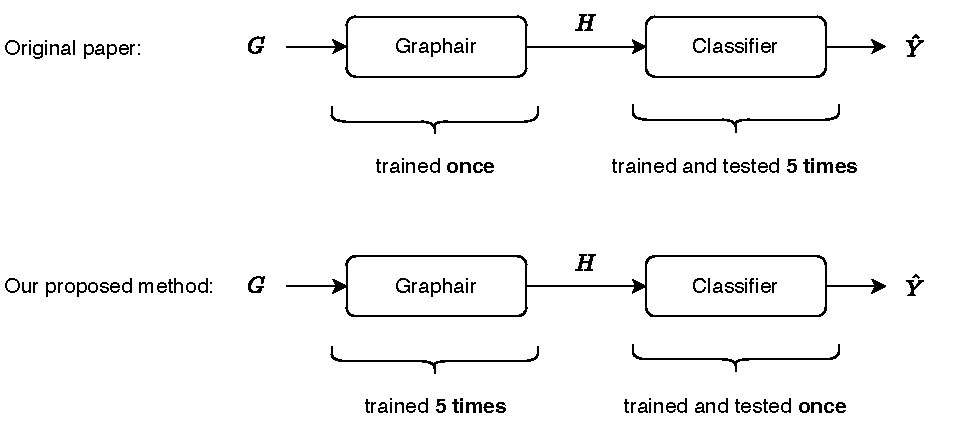
\includegraphics[scale=0.7]{images/evaluation-protocol.pdf}
    \caption{Evaluation protocol of the original paper and our proposed method.}
    \label{fig:enter-label}
\end{figure}

\section{Grid Search Best Accuracy Results}\label{appendix:best-accuracy}


\begin{table}[H]
    \caption{Best-accuracy results on the NBA, Pokec-z, and Pokec-n datasets, showing the original ones, the reproduced results with an identical experimental setup, and the results employing our proposed evaluation protocol.}
    
    \label{tab:reproduction-nba}
    \centering
    \resizebox{\textwidth}{!}{
    \begin{tabular}{llccc}
        \bf DATASET & \multicolumn{1}{c}{\bf SETTING} & \bf ACCURACY $\uparrow$ & $\Delta$ \bf DP $\downarrow$ & $\Delta$ \bf EO $\downarrow$ \\
        \hline\\
        \multirow{3}*{NBA} & original (original evaluation protocol) & $69.36 \pm 0.45$ & $\mathbf{2.56} \pm \mathbf{0.41}$ & $4.64 \pm 0.17$\\
        & reproduction (original evaluation protocol) & $\mathbf{70.92 \pm 1.19}$ & $18.50 \pm 5.32$ & $9.30 \pm 3.63$\\
        & reproduction (our evaluation protocol) & $70.35 \pm 0.53$ & $4.75 \pm 2.60$ & $\mathbf{4.55 \pm 1.95}$\\\\
        \hline\\
        \multirow{3}*{Pokec-z} & original (original evaluation protocol) & $\mathbf{68.17 \pm 0.08}$ & $\mathbf{2.10} \pm \mathbf{0.17}$ & $\mathbf{2.76 \pm 0.19}$\\
        & reproduction (original evaluation protocol) & $62.01 \pm 0.03$ & $3.74 \pm 0.69$ & $4.93 \pm 1.01$\\
        & reproduction (our evaluation protocol) & $60.94 \pm 2.34$ & $3.73 \pm 1.43$ & $4.36 \pm 2.68$\\\\
        \hline\\
        \multirow{3}*{Pokec-n} & original (original evaluation protocol) & $\mathbf{67.43 \pm 0.25}$ & $\mathbf{2.02 \pm 0.40}$ & $\mathbf{1.62 \pm 0.47}$ \\
        & reproduction (original evaluation protocol) & $63.59 \pm 0.30$ & $3.80 \pm 0.43$ & $3.83 \pm 0.60$\\
        & reproduction (our evaluation protocol) & $62.79 \pm 1.41$ & $5.48 \pm 2.62$ & $4.73 \pm 1.87$\\
    \end{tabular}}
\end{table}

\section{Pareto-Fronts of Grid Searches}\label{appendix:pareto-fronts}

\begin{figure}[H]
    \centering
    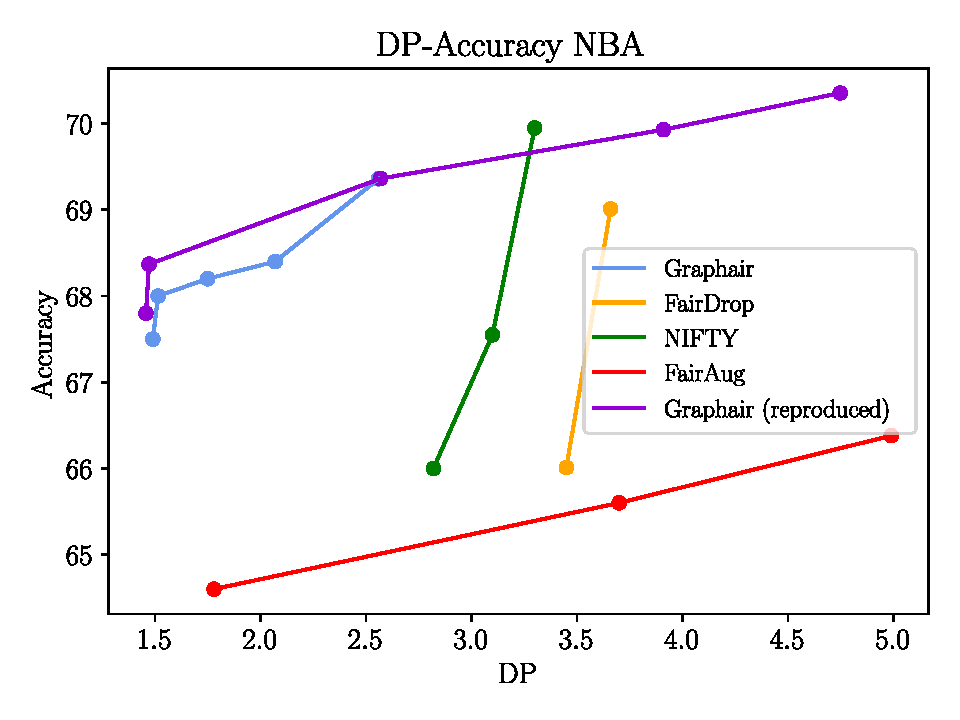
\includegraphics[width=0.32\textwidth]{images/DP_ACC_NBA.pdf}
    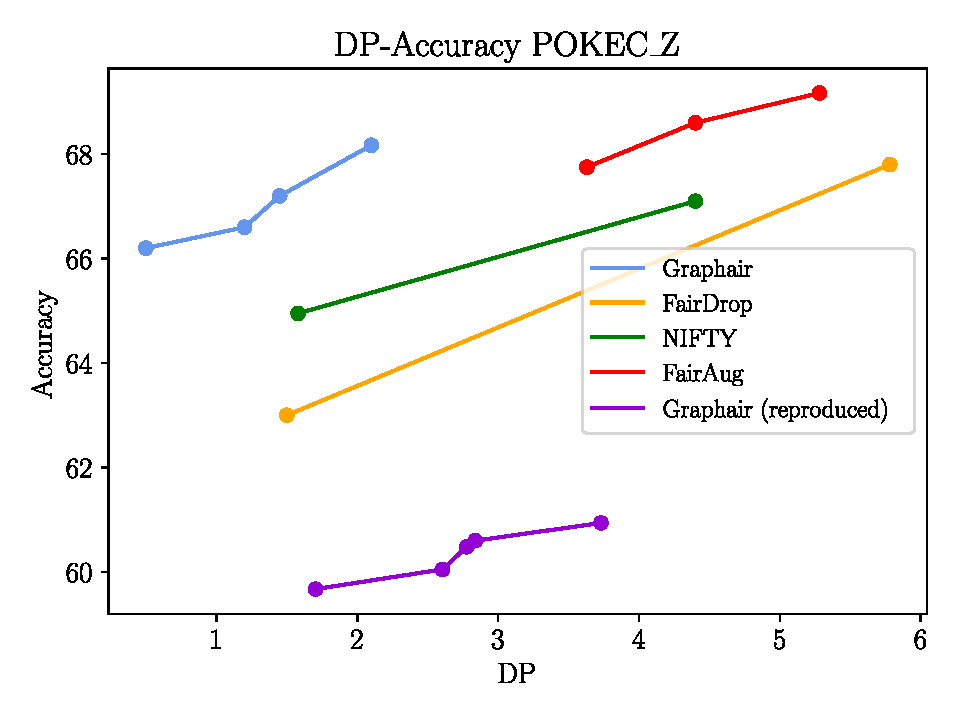
\includegraphics[width=0.32\textwidth]{images/DP_ACC_POKEC_Z.pdf}
    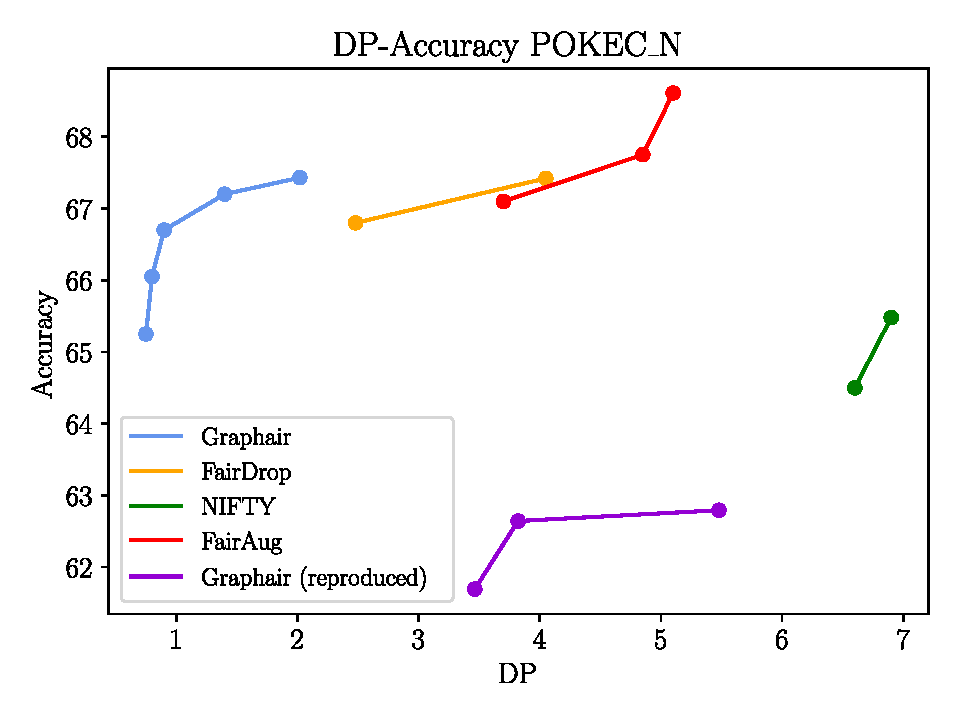
\includegraphics[width=0.32\textwidth]{images/DP_ACC_POKEC_N.pdf}
    \caption{DP-Accuracy Pareto front plots for all three datasets. Graphair (reproduced) refers to the model trained with our proposed evaluation protocol.}
    \label{fig:pareto-fronts}
\end{figure}

\section{Original Framework}

\begin{figure}[H]
    \centering
    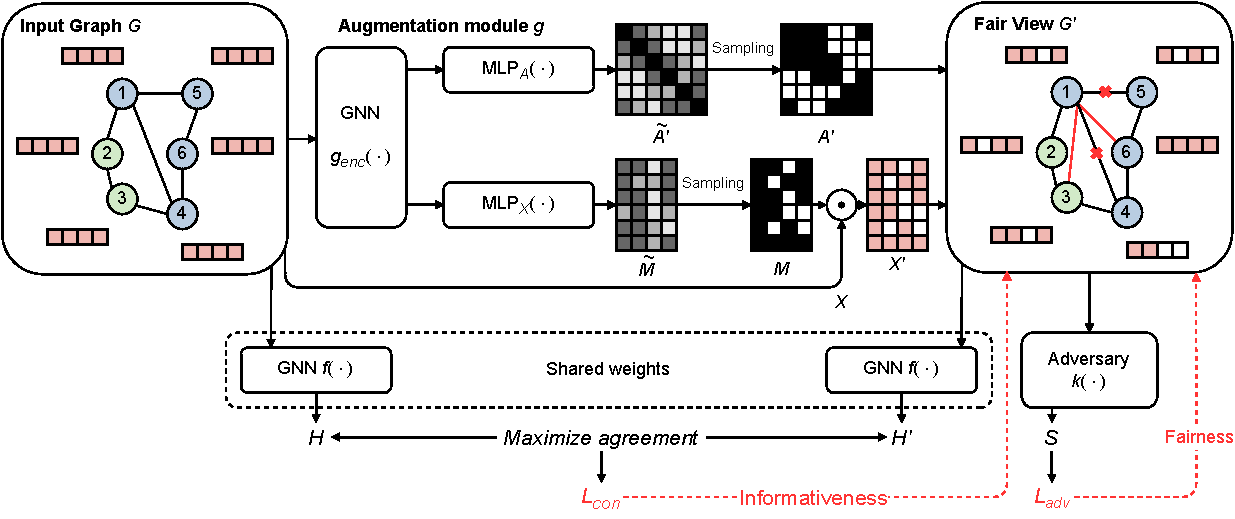
\includegraphics[width=\textwidth]{images/GraphAir.pdf}
    \caption{Graphair framework. The graphic was adapted from the original paper \citep{ling2023learning}.}
    \label{fig:original-framework}
\end{figure}

\section{Framework for Ablation Study}

\begin{figure}[H]
    \centering
    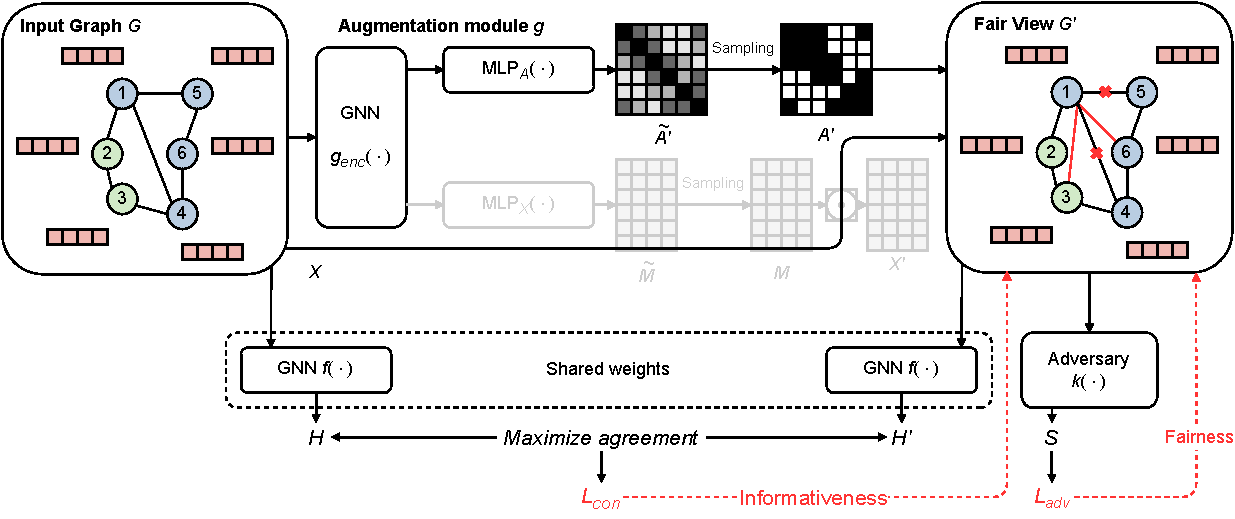
\includegraphics[width=\textwidth]{images/GraphAirAblation.pdf}
    \caption{Graphair framework without node feature masking for the ablation study.}
    \label{fig:ablation}
\end{figure}

\section{Framework without Adversarial Training}

\begin{figure}[H]
    \centering
    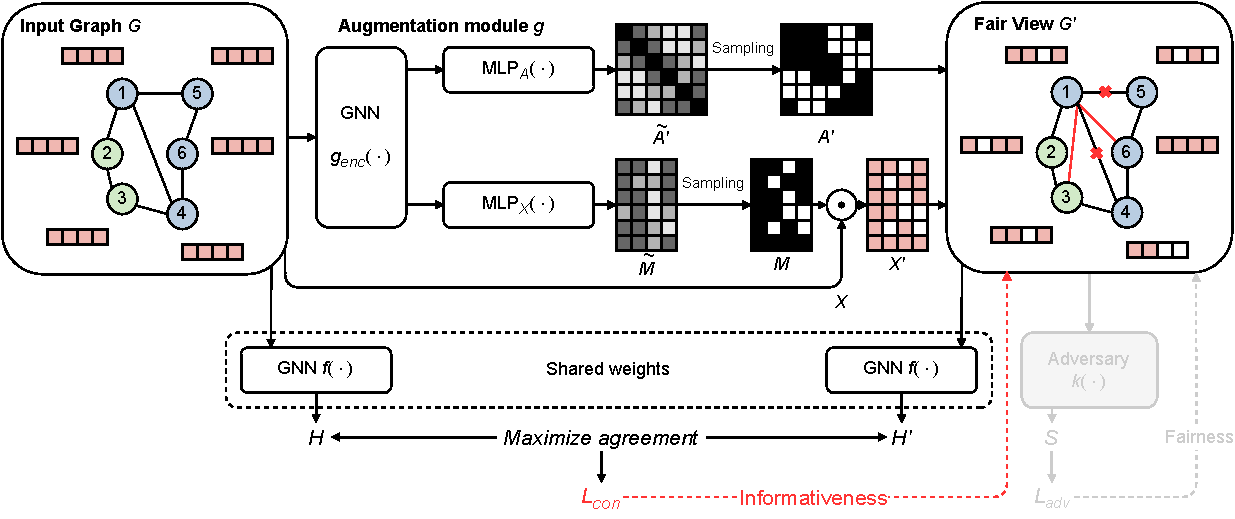
\includegraphics[width=\textwidth]{images/GraphAirNo Adversary.pdf}
    \caption{Graphair framework without the adversarial training.}
    \label{fig:without-adversarial}
\end{figure}


\section{Framework for Supervised Training}

\begin{figure}[H]
    \centering
    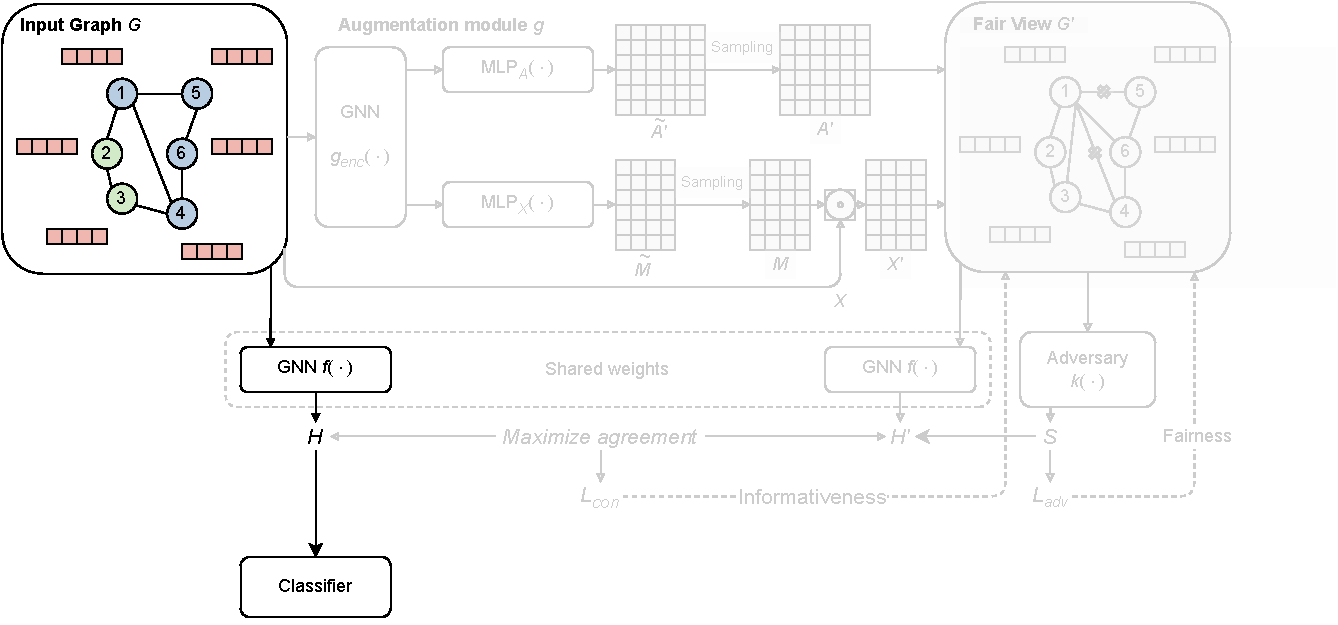
\includegraphics[width=\textwidth]{images/GraphAirSupervised.pdf}
    \caption{Fully-supervised training without Graphair framework.}
    \label{fig:supervised}
\end{figure}

\section{Further Explanations on Homophily}\label{appendix:homophily}

Homophily refers to the tendency of similar nodes to connect \citep{mcpherson2001birds}. Hence, the probability that two nodes $i$ and $j$ connect is determined by the homophily value between their classes $c_i$ and $c_j$, where a value lower than $0.5$ means that $i$ is more likely to connect to a node from a different class than $c_j$, and a value higher than $0.5$ means that $i$ is more likely to connect to a node of class $c_j$ than other classes. The specific definition of the corresponding probabilities is defined in the work by \citet{espin2022inequality}.
Since we use two groups, i.e., majority $M$ and minority $m$, there are two homophily settings: $h_{MM}$ referring to the tendency of majority group nodes connecting to each other, and $h_{mm}$ referring to how much minority groups tend to connect to each other. 
Note that the between-group connectivity values are determined correspondingly: $h_{mM} = 1 - h_{mm}$ and $h_{Mm} = 1 - h_{MM}$.

\section{Additional Results for Scaled Training Runs}

In addition to repeating the experiments on the Pokec datasets with corrected step counts ($11,000$ instead of $500$), we perform experiments with larger batch sizes. These are performed using the initial step count in light of computational resource limits. Moreover, due to the maximum memory capacity of the utilized GPU of $40$GB, the largest possible batch size we could fit was $2000$.\\
The results are shown in Table \ref{tab:scaled-results} alongside the ones for larger step counts. Larger batch size generally performs worse on accuracy, DP, and EO. However, on Pokec-z, a lower DP is achieved compared to the other large-scale run.

\begin{table}[H]
    \caption{Results for our scaled training runs on the Pokec datasets with significantly larger epoch count and batch size. The NBA dataset is omitted as its small size makes an analogous run superfluous.}
    
    \label{tab:scaled-results}
    \centering
    \begin{tabular}{lccccc}
        \bf DATASET & 
        \textbf{BATCH SIZE} & 
        \bf EPOCHS &
        \bf ACCURACY &
        $\Delta$ \bf DP $\downarrow$ & 
        $\Delta$ \bf EO $\downarrow$\\
        \hline\\

        Pokec-z & $1000$ & $11000$ & $63.39 \pm 0.68$ & $2.28 \pm 1.52$ & $2.24 \pm 1.99$\\

        Pokec-z & $2000$ & $500$ & $60.46 \pm 2.58$ & $1.84 \pm 0.26$ & $2.56 \pm 1.00$\\

        Pokec-n & $1000$ & $11000$ & $63.88 \pm 0.91$ & $2.85 \pm 0.59$ & $2.40 \pm 0.11$\\

        Pokec-n & $2000$ & $500$ & $62.59 \pm 1.30$ & $5.85 \pm 0.65$ & $5.31 \pm 1.23$\\
    \end{tabular}
\end{table}